
\documentclass{beamer}
\usepackage{ucs}
\usepackage[utf8x]{inputenc}
\usepackage[T1]{fontenc}

\usepackage{graphicx}
\usepackage{tipa}

\begin{document}
\title{Interactive Pedagogical Programs Based on Constraint Grammar}   
%\author{Lene Antonsen\\ Saara Huhmarniemi\\Trond Trosterud\\ University of Tromsø\\Norway
\author{Lene Antonsen, Saara Huhmarniemi, Trond Trosterud \\
Centre for Sámi Language Technology \begin{figure}  \scalebox{0.10}[0.10]{
\includegraphics{img/LogoEngelsk}} \end{figure} 
}
\date


\frame{\titlepage} 

%\frame{\frametitle{Contents}\tableofcontents} 


%\section{1. Introduction} 

\frame{\frametitle{Parser-based CALL programs}
Parser-based CALL programs for learners of North Sámi based on pre-existing LT resources developed at the University of Tromsø:
\begin{itemize}
\item finite state morphological analyser/generator (fst)
\item constraint grammar (CG) parser
\item number word generator (xfst)
\end{itemize} 
%(Trosterud 2007) \\
\vspace{0.5cm}
The morphological analyser/generator is implemented with fst and compiled with the Xerox compilers twolc and lexc. \\ %(Beesley and Karttunen 2003). \\
The morphological disambiguator is implemented in the CG-framework. %(Karlsson et al 1995).
}


\frame{\frametitle{Previous accounts on parser-based CALL}
Very few parser-based CALL (Computer Assisted Language Learning) programs are available for actual use online. \pause We have looked at 
\begin{itemize}
\item \textbf{e-tutor}, a program for teaching German to foreigners at \textit{http://e-tutor.org/} with Head-driven Phrase Structure Grammar (HPSG). e-tutor gives very good feedback to student's errors, but the possible input is very restricted. \pause %(Heift 2001, Heift and Nicholson 2001). \pause
\item \textbf{VISL}-suite of games for teaching grammatical analysis at \textit{http://visl.sdu.dk/} with vislcg3. One of the programs accepts free user input. The input is analysed or changed into grammar exercises. %(Bick 2005).
\end{itemize}
%(Gamper and Knapp 2001, Heift and Schulze 2007)
}


%\frame{\frametitle{Pedagogical motivation of OAHPA!}
%To develop a language tutoring system which
%\begin{itemize}
%\item has free-form dialogues and sophisticated error analysis
%\item gives immediate error feedback and advice to the user
%\item is flexible
%\item is easily integrated to the instruction in school and university
%\item make it possible to choose main dialect and metalanguage
%\item is freely accessible via Internet
%\end{itemize}
%
%}
%
%
%
\frame{\frametitle{http://oahpa.uit.no/} 
\scalebox{0.30}[0.30]{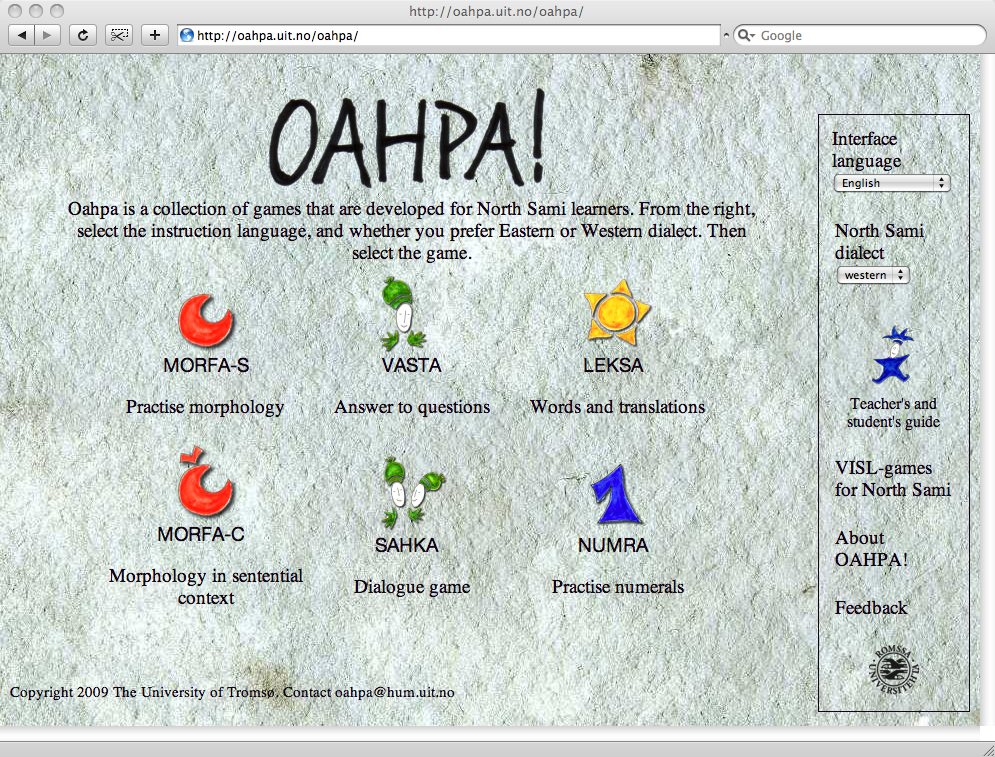
\includegraphics{img/Oahpanew.png}} \\
}
%
%
%%\section{2. Pedagogical lexicon} 
%
%
%\frame{\frametitle{Pedagogical lexicon} 
%\scalebox{0.40}[0.40]{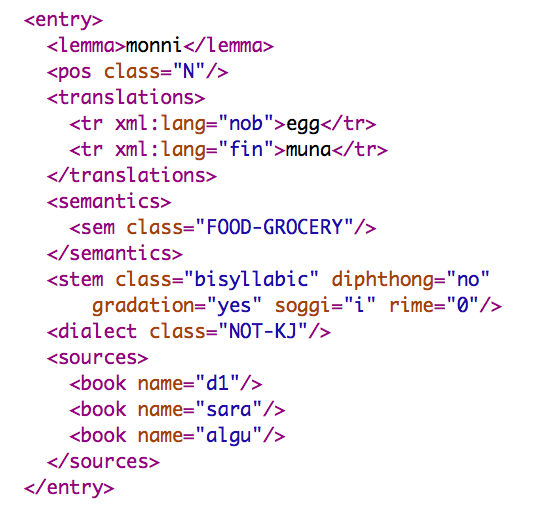
\includegraphics{img/nounlexiconMonni.png}} \\
%}
%
%
%\frame{\frametitle{Dialectial variation} 
%NOT-KJ (not generated for KJ-dialect) \\
%NOT-GG (not generated for GG-dialect) \\  
%\vspace{1cm} \pause
%\scalebox{0.60}[0.60]{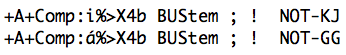
\includegraphics{img/smelex3.png}} \\
%\vspace{0.5cm}
%\textit{stuoris} $\rightarrow$ \textit{stuorit} (NOT-KJ) vs. \textit{stuorát} (NOT-GG) ("big")
%}
%
%
%\frame{\frametitle{System for morphological feedback} 
%\scalebox{0.50}[0.50]{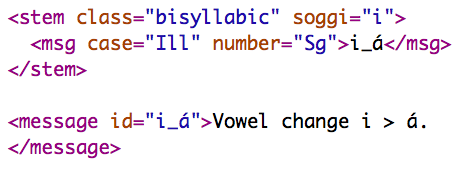
\includegraphics{img/morphfeedbackEngColours.png}} \\
%}
%
%\frame{\frametitle{Morphological feedback} 
%used in \textbf{Morfa-S} -- basic morphological exercises\\
%\vspace{1.0cm}
%\scalebox{0.80}[0.80]{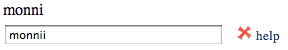
\includegraphics{img/monniiwindow.png}} \\ \pause
%\vspace{0.5cm}
%\scalebox{0.80}[0.80]{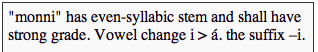
\includegraphics{img/monnifeedbackwindow.png}} \\ \pause
%\vspace{0.5cm}
%\scalebox{0.80}[0.80]{
\includegraphics{img/monniwindowCorr.png}} \\
%}

%\frame{\frametitle{Sentence generator} 
%used in \textbf{Vasta} -- the question-answer drill and in \textbf{Morfa-C} -- morphological exercises in a sentential frame \\
%\vspace{0.5cm}
%\scalebox{0.50}[0.50]{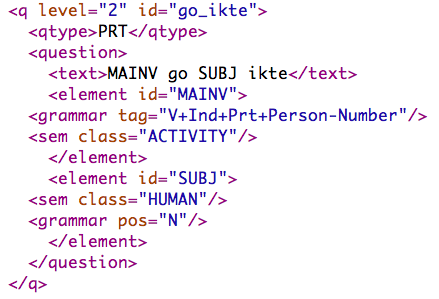
\includegraphics{img/sentencegenerator.png}} \\
%\vspace{0.5cm}
%(MAINV question-particle SUBJ yesterday)
%}

\frame{\frametitle{Vasta -- QA drill with sentence generator} 
\scalebox{0.50}[0.50]{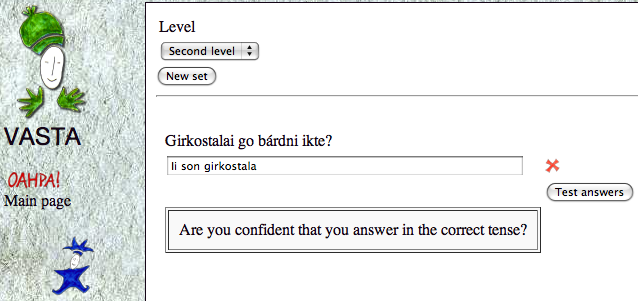
\includegraphics{img/Vasta_sentencegen_example.png}} \\
\vspace{0.5cm}
("Did the boy go to church yesterday?" \\
"No, he does not.")
}

\frame{\frametitle{Sahka -- dialogue program with tailored questions} 
\scalebox{0.39}[0.41]{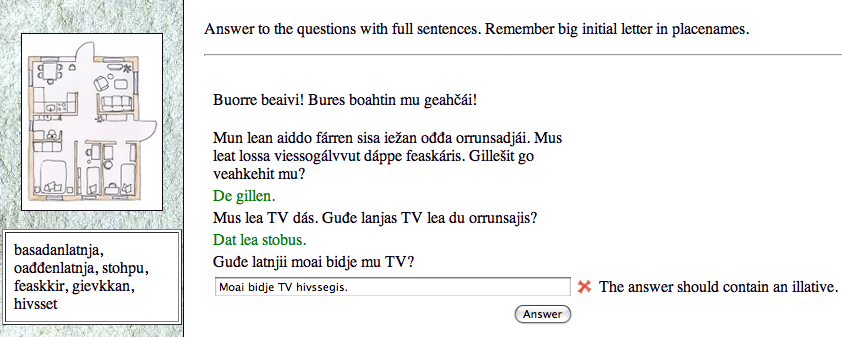
\includegraphics{img/TVhivssegis.png}} \\ 
\vspace{0.5cm}
(Question: "In which room should we place the TV?" \\
Answer: "We should place it in the toilet.")
}



%\section{2. CG-parser in live analysis}
\frame{\frametitle{Constraint Grammar parser -- vislcg3}
%CG is robust enough for handling unconstrained input, and at the same time accurate enough to identify errors. \\
%\vspace{0.4cm}
\begin{itemize}
\item consists of manually written, context dependent rules which
add, remove, select or replace tags or sets of grammatical tags in a given sentential context. \pause
\item context conditions may be linked to any tag or tag set of any word anywhere in the sentence, either locally (in a fixed subdomain of the context) or globally (in the whole context). \pause
\item context conditions in the same rule may be linked, i.e. conditioned upon each other, negated or blocked by interfering words or tags.  \\
\end{itemize}
\vspace{0.4cm}
Grammars for Danish and Norwegian based on CG achieve very good F-scores. \\
%\vspace{0.4cm}
%(Bick 2003, VISL-group 2008) \\

}


%\frame{\frametitle{multi} 
%\scalebox{0.90}[0.90]{\includegraphics{multi.png}} \\
%}
%
%\frame{\frametitle{dis} 
%\scalebox{0.90}[0.90]{\includegraphics{dis.png}} \\
%}


\frame{\frametitle{Schematical view of the process} 
\scalebox{0.55}[0.55]{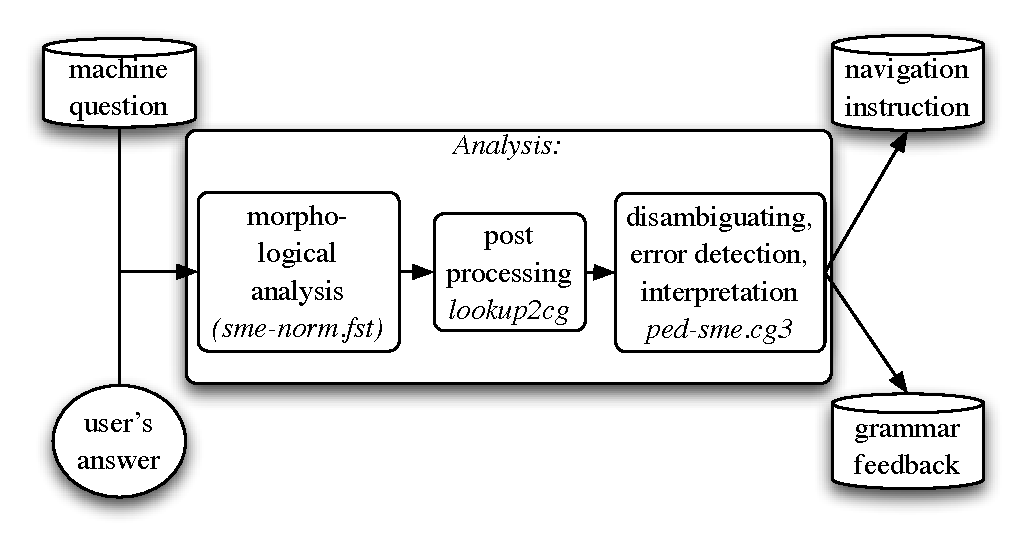
\includegraphics{img/qa2.pdf}} \\
}


\frame{\frametitle{Morphological analysis} 
\scalebox{0.35}[0.35]{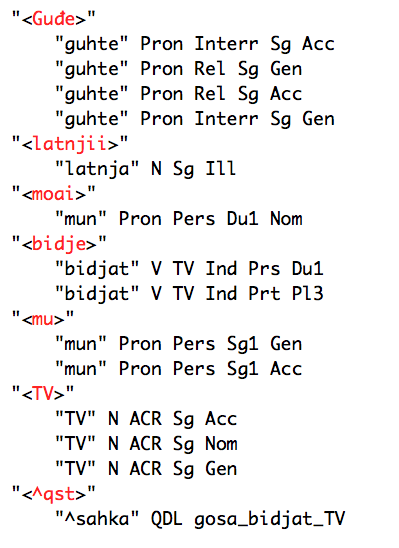
\includegraphics{img/GudelatnjiiQ.png}{img/GudelatnjiiB.png}}\scalebox{0.35}[0.35]{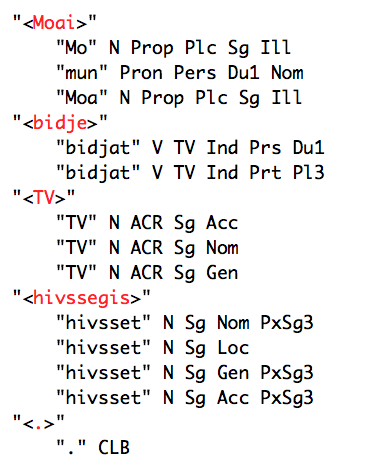
\includegraphics{img/GudelatnjiiA.png}{img/GudelatnjiiB.png}} \\
}



%\frame{\frametitle{multi} 
%\scalebox{0.38}[0.38]{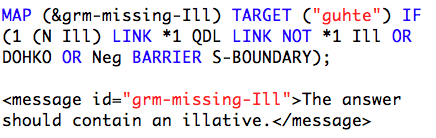
\includegraphics{img/missingIll.png}} \\
%}

%The most difficult problem for the grammatical analysis are the student's misspellings. A misspelling may be left unrecognized in the analysis or it can produce another word form for the same lemma, or from some other lemma. 
%
%When the word form is not recognized during the analysis, the feedback message to the student points to the unrecognized word form asking the student to check the spelling. To the extent that misspellings are the most common type of errors, the current feedback does not provide enough instructions for the student to improve the spelling. However, in order to give better feedback to certain misspellings, we have added e.g. place names with small initial letter to the fst, together with an error tag, so that the student gets a precise feedback. We will implement more that kind of rules and consider usage of a spell checker to help the student to find the correct word form.
%
%%\textit{The word form is not in our lexicon, can it be a spelling error?}. 
%% sh: let's give examples of something that we can do well.
%
%For misspellings that produce another word form of the same lemma, we have written rules that are based on the grammatical context. The real problem emerges when the spelling error gives rise to an unintended lemma. Then the challenge is to give a feedback according to what the student thinks she has written. In this case, feedback has to be tailored using the knowledge about the student’s interlanguage. We have created sets for typical unintended lemmata. Combined with contextual rules we can then give the user a good feedback due to the misspelling instead of the unintended lemma.
%
%E.g. if the student uses the Sg2 form of the main verb after the negative verb, instead of the correct ConNeg form, then the erroneous form can be a ConNeg form of a derivated verb, and the normal feedback will be: "You should answer with the same verb as in the question." The student will not understand this, because she thinks that the word form in the answer is an instance of the same verb. The solution was to generate all these forms of the verbs in the questions, make a set of them, and make a rule for in the right context, give the feedback: "The negative form is not correct." 

\frame{\frametitle{Assigning of navigation tag} 
\scalebox{0.3}[0.3]{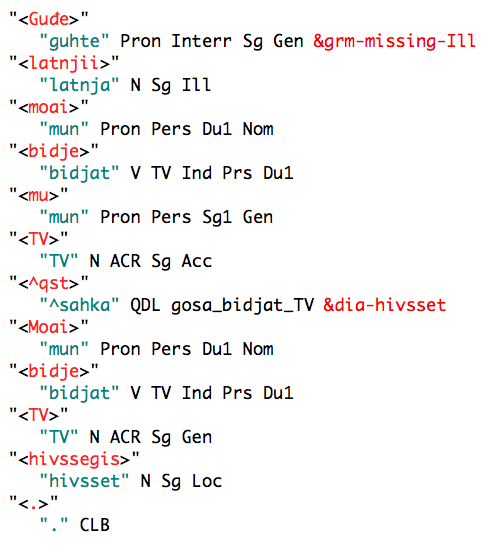
\includegraphics{img/hivssegisCGanal.png}} \\
\vspace{0.5cm}
\scalebox{0.3}[0.3]{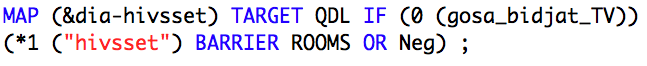
\includegraphics{img/hivsset_tag.png}} \\
}
\frame{\frametitle{Navigating in the dialogue -- alternative links} 
\scalebox{0.35}[0.35]{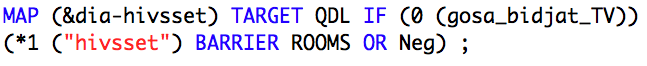
\includegraphics{img/hivsset_tag.png}} \\
\scalebox{0.55}[0.55]{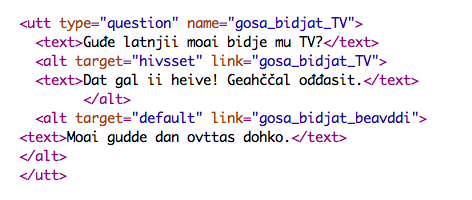
\includegraphics{img/gosabidjatTV.png}} \\
Question: "In which room should we place the TV?" \\
Alt. WC: "That is not a good idea. Make a new try." \\ 
Default: "We carry it there together." 
}

\frame{\frametitle{Navigating in the dialogue -- alternative branches} 
\scalebox{0.45}[0.45]{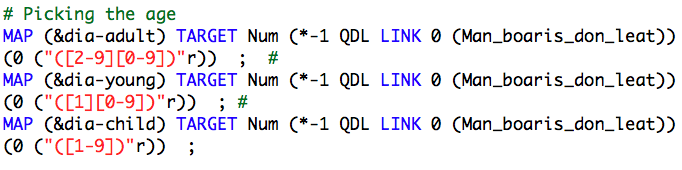
\includegraphics{img/pickingage_colours.png}} \\
\vspace{0.5cm} \pause
\scalebox{0.45}[0.45]{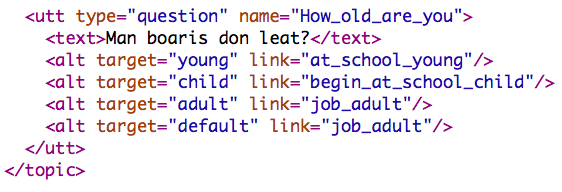
\includegraphics{img/age_branching.png}} \\
("How old are you?")
}

\frame{\frametitle{Disambiguation and assigning of grammar tag} 
\scalebox{0.3}[0.3]{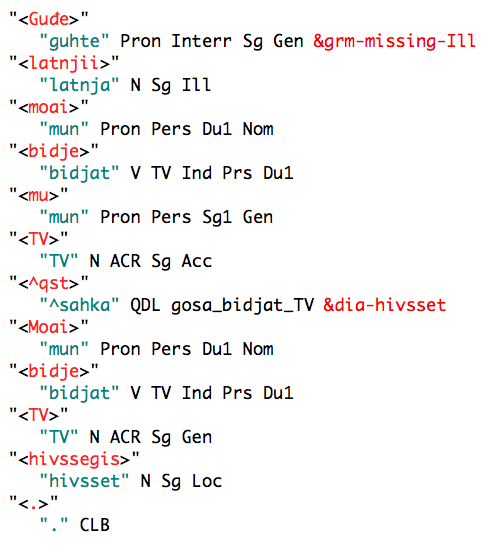
\includegraphics{img/hivssegisCGanal.png}} \\
\scalebox{0.35}[0.35]{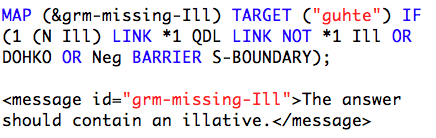
\includegraphics{img/missingIll.png}} \\
}




\frame{\frametitle{The grammar errors we have rules for 1} 
Verbs and their arguments
\begin{itemize}
\item verbs: finite, infinite, negative form, correct person/tense according to the question
\item case of argument based upon the interrogative 
\item case of argument based upon valency
\item locative vs. illative based upon movement
\item subject/verbal agreement
\end{itemize}
}

\frame{\frametitle{The grammar errors we have rules for 2} 
Other
\begin{itemize}
\item agreement inside NP 
\item numeral expressions: case and number  
\item PP: case of noun, pp based upon the interrogative  
\item time expressions 
\item special adverbs  
\item particles according to word order 
\item comparision of adjectives
\end{itemize}
}

\frame{\frametitle{Meta comments} 
\begin{itemize}
\item "Answering \textit{I-don't-know} is too simple. Try again."
\item "Your answer must always contain a finite verb. Could there be a typo in the verbform?"
\item "You must use one of the words in the wordlist in the left margin."
\item "You have not used the correct adjective. Try again." 
\item The user can quit the dialogue in a proper way by using the verb "heaitit" (= to quit) -- then the system navigates to the closing utterance of the dialogue (to be implemented)
\end{itemize}
%\hspace{0.5cm} \scalebox{0.45}[0.45]{
\includegraphics{img/diastop.png}} \\

}


%\section{3. Evaluation}
\frame{\frametitle{Evaluation: The actual use}
The programs are free available at internet. Appr. 500 queries/day. \\
\begin{table}
\begin{tabular}{|c|c|c|c|c|c|}
\hline
Morfa-S & Leksa & Sahka & Numra & Morfa-C & Vasta \\
41\% & 27\% & 13\% & 12\% & 5\% & 2\% \\
\hline
\end{tabular}
\end{table}
}

\frame{\frametitle{Evaluation: How the rules have been working}
The system has identified an error in the user's input:
\begin{table}
\begin{tabular}{|l|c|c|c|}
\hline 
\textbf{Rule type}  & \textbf{correct} & \textbf{wrong}   & \textbf{corr. \% }  \\
\hline 
wrong tense         & 7     & 0     & 100,0     \\ 
wrong V after neg   & 3     & 0     & 100,0     \\ 
no infinite V       & 1     & 0     & 100,0     \\ 
\hline 
orth. error         & 44    & 2     & 95,7      \\
wrong case for V-arg  & 26    & 4     & 86,7      \\
no finite verb        & 19    & 4     &  82,6 \\
\hline 
wrong S-V agreement   & 17    & 8     & 68,0 \\
wrong V choice        & 7     & 4     & 63,6 \\
\hline 
wrong word            & 4     & 4     & 50,0 \\
wrong case after Num  & 1     & 1     & 50,0 \\
\hline
\end{tabular}
\end{table}
Misspellings a problem for the user
}

%\frame{\frametitle{Evaluation 3}
%Which rules are not in use? Why? \\
%\begin{itemize}
%\item agreement inside NP (except for numeral expressions)
%\item PP: case of noun, pp based of the interrogative  
%\item time expressions 
%\item particles according to word order 
%\end{itemize}
%
%}
%
%
%\frame{\frametitle{An alternative to free input: the German e-tutor} 
%\scalebox{0.45}[0.45]{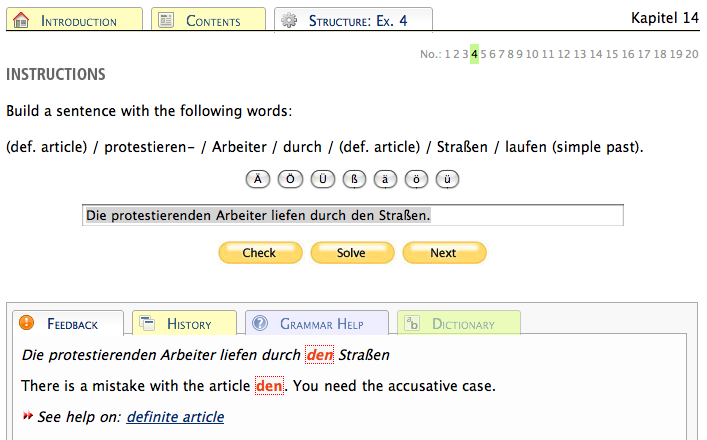
\includegraphics{img/e-tutor.png}} \\
%}

\frame{\frametitle{Evaluation: Precision and recall -- today}
\begin{table}%[htdp]
%\caption{default}
%\begin{center}
\begin{tabular}{|l|r|r|r|r||r|r|r|r|r|}
\hline
Error type	& tp		& fp		& tn		& fn	& prec	 & rec.	& acc.	& F-ms. \\
\hline
Gramm. err.   &   641   &   234   &   769    &   7    &   0,73   &   0,99   &   0,85   &   0,84	  \\
Sem. err.     &   805   &   69    &   764    &   12   &   0,92   &   0,99   &   0,95   &   0,95		  \\
Orth. err     &   875   &   0     &   776    &   0    &   1      &   1      &   1      &   1					  \\
Other err.    &   695   &   180   &   751    &   25   &   0,79   &   0,97   &   0,88   &   0,87	  \\
\hline
  &   3016  &   483   &   3060   &   44   &   0,86   &   0,98   &   0,92   &   0,92			  \\
\hline
\end{tabular}
%\end{center}
%\label{default}
\end{table}%

The high recall compared to the somewhat lower precision indicates that the system is a bit too critical towards the students:
\begin{itemize}
\item{It almost never lets through a (targeted) mistake, with the price of flagging some correct answers as errors.}
\end{itemize}
}


%%\section{7. Future perspectives}
%\frame{\frametitle{Future perspectives}
%How to improve the system? \\
%\begin{itemize}
%\item speller for misspellings 
%\item grammartasks a la \textit{e-tutor}?
%\item Vasta: decide what words the user should use, ala e-tutor as a supplement
%\item Vasta: the user can choice topic instead of grammar tasks
%\item Make the programs for more sámi languages
%\item Classroom studies
%\end{itemize}
%
%}




%%\section{4. Conclusion}
%\frame{\frametitle{Conclusion}
%
%\begin{itemize}
%\item By using a sloppy version of the syntactical analyser for North Sámi, combined with a set of error-detection rules, we have been able to build a flexible CALL resource. \\ \pause
%\item The precision is not good enough
%\item We need some kind of speller or a sloppy fst with errortags
%\item "Totally" free input not always the best
%\end{itemize}
%}

%\frame{\frametitle{Thanks to} 
%The faculty of Humanities at the University of Tromsø, and the Sámi Parliament in Norway, for funding the project. \\
%} 
%
%\frame{\frametitle{Centre for Sámi Language Technology} 
%http://giellatekno.uit.no/ \\
%http://oahpa.uit.no/
%
%} 


%%\section{4. Evaluation}
%\frame{\frametitle{Evaluation 1}
%Answers to the programs (Vasta and Sahka were logged at the end of the period only).
%\begin{table}
%\begin{center}
%\begin{tabular}{|l|r|r|r|r|}
%\hline
%Program     & Correct &   Wrong &    Total &  \% \\
%\hline									 
%Morfa-S  &  6920   & 6323    & 13243    & 52.3 \\
%Leksa    &  5659   & 4248    & 9907	    & 57.1  \\
%Numra    &  3086   & 2512    & 5598	    & 55.1  \\
%Morfa-C  &  1349   & 1613    & 2962	    & 45.5  \\
%Sahka    &   322   &   322   &  644	    & 50.0  \\
%Vasta    &   19    &   102   &  121	    & 15.7 \\
%\hline
%Total   & 17355  &  15120  &  32475  &  53,44\\
%\hline
%\end{tabular}
%\end{center}
%\end{table}
%}
%
%\frame{\frametitle{Evaluation 2}
%Error types for Sahka, ordered after type.
%\begin{table}
%\begin{center}
%\begin{tabular}{|l|r|l|r|}
%\hline
%Error type & \# & Error type & \# \\
%\hline												    
%no finite verb    & 85 & wrong case for V-arg & 22  \\
%orth. error       & 83 & wrong case after Num & 10 \\
%wrong S-V agr     & 46 & wrong tense          & 9 \\
%no infinite V  & 30 & no postposition      & 6 \\
%wrong V choice & 24 & wrong word           & 7  \\
%\hline
%\end{tabular}
%\end{center}
%\end{table}
%Sahka and Vasta: Precision = 0.85; Recall = 0.93; \\ Accuracy = 0.89 (N=277).
%}
%

%\section{4. Conclusion}
\frame{\frametitle{Conclusion}
\begin{itemize}
\item A sloppy version of the syntactical analyser for North Sámi, combined with a set of error-detection rules, we have been able to build a flexible CALL resource. \\ \pause
\vspace{0.5cm}
\item The present project has shown that CG is well fit for making pedagogical dialogue systems.\\ \pause
\vspace{0.5cm}
\item The program suite is something quite new among pedagogical programs for Sámi, and indeed its dialogue and open QA-programs are quite rare within the field of parser-based CALL.
\end{itemize}
}

\frame{\frametitle{Acknowledgments} 
Thanks to the faculty of Humanities at the University of Tromsø, and the Sámi Parliament in Norway, for funding the project.} 

\frame{\frametitle{Centre for Sámi Language Technology} 
http://giellatekno.uit.no/ \\
http://oahpa.uit.no/

} 


%\frame{\frametitle{References} 
%\scalebox{0.32}[0.32]{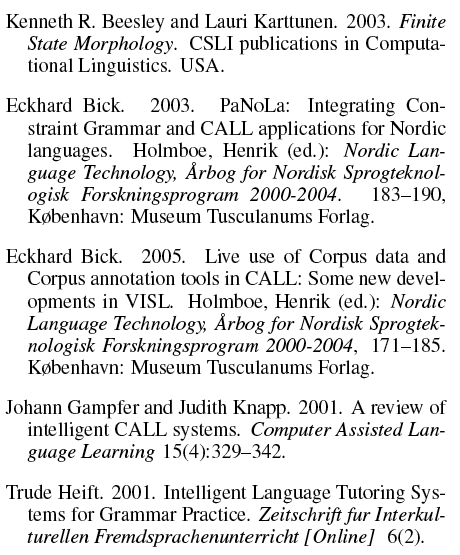
\includegraphics{img/ref1.png}}
%\scalebox{0.32}[0.32]{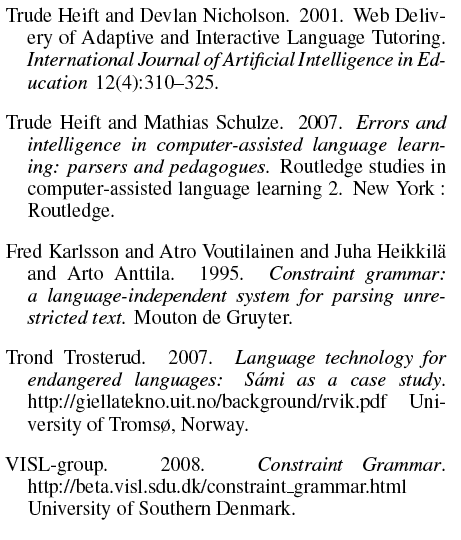
\includegraphics{img/ref2.png}}
%} 

%\frame{\frametitle{References} 
%\small{\textbf{Beesley, K. and L. Karttunen. 2003.} Finite
%State Morphology. CSLI publications in Computational
%Linguistics. USA.\\
%\textbf{Bick, E. 2003.} PaNoLa: Integrating Constraint
%Grammar and CALL applications for Nordic
%languages. Holmboe, Henrik (ed.): Nordic Language
%Technology, Årbog for Nordisk Sprogteknologisk
%Forsknings- program 2000-2004. 183–190,
%København: Museum Tusculanums Forlag.\\
%\textbf{Bick, E. 2005.} Live use of Corpus data and
%Corpus annotation tools in CALL: Some new developments
%in VISL. Holmboe, Henrik (ed.): Nordic
%Language Technology, Årbog for Nordisk Sprogteknologisk
%Forsknings- program 2000-2004, 171–185.
%København: Museum Tusculanums Forlag.\\
%\textbf{Johann Gampfer and Judith Knapp. 2001.} A review of
%intelligent CALL systems. Computer Assisted Language
%Learning 15(4):329–342.\\
%\small{\textbf{Trude Heift. 2001.} Intelligent Language Tutoring Systems
%for Grammar Practice. Zeitschrift fur Interkulturellen
%Fremdsprachenunterricht [Online] 6(2).\\
%\textbf{Trude Heift and Devlan Nicholson. 2001.} Web Delivery
%of Adaptive and Interactive Language Tutoring.
%International Journal of Artificial Intelligence in Education
%12(4):310–325.\\
%\textbf{Trude Heift and Mathias Schulze. 2007.} Errors and
%intelligence in computer-assisted language learning:
%parsers and pedagogues. Routledge studies in
%computer-assisted language learning 2. New York :
%Routledge.\\
%\textbf{Karlsson, F., A. Voutilainen, J. Heikkilä
%and A. Anttila. 1995.} Constraint grammar:
%a language-independent system for parsing unrestricted
%text. Mouton de Gruyter.\\
%\textbf{Trosterud, T. 2007.} Language technology for
%endangered languages: Sámi as a case study.
%http://giellatekno.uit.no/background/rvik.pdf University
%of Tromsø, Norway.\\
%\textbf{VISL-group. 2008.} Constraint Grammar.
%http://beta.visl.sdu.dk/ constraint grammar.html
%University of Southern Denmark.
%}} 
%

%\frame{\frametitle{References 1} 
%\small{Kenneth R. Beesley and Lauri Karttunen. 2003. Finite
%State Morphology. CSLI publications in Computational
%Linguistics. USA.\\
%Eckhard Bick. 2003. PaNoLa: Integrating Constraint
%Grammar and CALL applications for Nordic
%languages. Holmboe, Henrik (ed.): Nordic Language
%Technology, Årbog for Nordisk Sprogteknologisk
%Forskningsprogram 2000-2004. 183–190,
%København: Museum Tusculanums Forlag.\\
%Eckhard Bick. 2005. Live use of Corpus data and
%Corpus annotation tools in CALL: Some new developments
%in VISL. Holmboe, Henrik (ed.): Nordic
%Language Technology, Årbog for Nordisk Sprogteknologisk
%Forskningsprogram 2000-2004, 171–185.
%København: Museum Tusculanums Forlag.\\
%Johann Gampfer and Judith Knapp. 2001. A review of
%intelligent CALL systems. Computer Assisted Language
%Learning 15(4):329–342.\\
%}}
%\frame{\frametitle{References 2} 
%\small{Trude Heift. 2001. Intelligent Language Tutoring Systems
%for Grammar Practice. Zeitschrift fur Interkulturellen
%Fremdsprachenunterricht [Online] 6(2).\\
%Trude Heift and Devlan Nicholson. 2001. Web Delivery
%of Adaptive and Interactive Language Tutoring.
%International Journal of Artificial Intelligence in Education
%12(4):310–325.\\
%Trude Heift and Mathias Schulze. 2007. Errors and
%intelligence in computer-assisted language learning:
%parsers and pedagogues. Routledge studies in
%computer-assisted language learning 2. New York :
%Routledge.\\
%Fred Karlsson and Atro Voutilainen and Juha Heikkil¨a
%and Arto Anttila. 1995. Constraint grammar:
%a language-independent system for parsing unrestricted
%text. Mouton de Gruyter.\\
%Trond Trosterud. 2007. Language technology for
%endangered languages: S´ami as a case study.
%http://giellatekno.uit.no/background/rvik.pdf University
%of Tromsø, Norway.\\
%VISL-group. 2008. Constraint Grammar.
%http://beta.visl.sdu.dk/constraint grammar.html
%University of Southern Denmark.
%}} 


%\frame{\frametitle{Questions?} 
%} 
%


\end{document}

